\documentclass[11pt]{article}
\usepackage[letterpaper,margin=1in]{geometry}
\usepackage{amsmath,amsthm,amssymb,latexsym}
\usepackage{alltt,enumerate}
\usepackage{tikz,pgfmath,algorithm,algorithmic}
\usepackage{appendix}
\usepgflibrary{shapes}
\usetikzlibrary{arrows,automata,backgrounds}

\usepackage[style=numeric]{biblatex}
\addbibresource{bibtex.bib}

\usepackage{hyperref}
\hypersetup{
    colorlinks=true,
    linkcolor=blue,    
    urlcolor=cyan,
}

\begin{document}

%% Macros %%
\newcommand\one{\textsf 1}
\newcommand\zero{\textsf 0}
\newcommand\cost{\mathcal C}
\newcommand\Prob{\text{Pr}}

%%\newtheorem{remark}{Remark}
%%\newtheorem{question}{Q}
\theoremstyle{remark}
\newtheorem{alg}{Algorithm}

\newtheorem{theorem}{Theorem}
\newtheorem{defn}{Definition}
\newtheorem{prop}{Proposition}

\setlength\parindent{0in}
\addtolength\parskip{1ex}
\setlength\fboxrule{.5mm}\setlength{\fboxsep}{1.2mm}
\newlength\courseheader
\setlength\courseheader\textwidth
\addtolength\courseheader{-4mm}
\parindent=0pt
\parskip=1ex

\begin{center}
\framebox{\parbox\courseheader{\large
CS6820 Algorithms\hfill December 17, 2021\\
Final Project \hfill G\"oktu\u{g} Saatcio\u{g}lu (gs724) \hfill Mark Moeller (mdm367)}}
\end{center}
\medskip

These notes explore the problem of sampling random spanning trees on graphs. The
focus will be to present and analyze Wilson's famous algorithm for this problem,
but we take some detours along the way.

We have also implemented the algorithms presented and run them on various
graphs. Details of our implementation are presented in Section~\ref{imp}.
As a 6820 final project, our approach is a hybrid of the ``Extra topic'' and ``Coding
project'' project types.

\section{Introduction: Spanning Trees}

In this section we introduce notation and explore basics of distributions on
spanning trees.

\subsection{Definitions}

\begin{defn}
For a connected undirected graph $G = (V, E)$, a collection of edges $T \subseteq E$
form a \emph{spanning tree} if $(V, T)$ is connected and acyclic.
\end{defn}

Suppose the edges have nonnegative costs given by a function $w\colon E \to
\mathbb{R^+}$, then the weight of a spanning tree is:
\[ w(T) = \prod_{e\in T} w(e) \]

\begin{defn}
A spanning tree for $G$ is called the \emph{minimum spanning tree} if it has the
minimum weight of all spanning trees of $G$.
\end{defn}

Prim's and Kruskal's algorithms are classic fast algorithms for finding minimum
spanning trees. Kozen gives an enlightening general framework that subsumes both
algorithms \cite{kozen}.

In some situations in distributed systems or networking, however, we may not
want the minimum spanning tree necessarily, but instead we want to sample
randomly from a distribution of spanning trees. We will present an algorithm due
to Wilson \cite{wilson} for doing this in Section~\ref{wilson}. Then we will see
how it can be extended to consider graphs with weights. In this case, the
probability of sampling a given tree will be proportional to its weight.

% Some stuff about how many trees there are?


\section{Naive First Attempt}\label{naive-attempt}

Before seeing Wilson's algorithm, which is based on random walks, we might be
tempted to try to sample random spanning trees by modifying Kruskal's algorithm.
That is:
\begin{itemize}
\item Choose a random order on edges, perhaps based on edge weights
\item Choose edges from the list in order, skipping an edge if it would make a
cycle
\end{itemize}

Unfortunately, we will not achieve the appropriate distributions following this
path. For a counterexample, consider the triangle graph $G = (\{a,b,c\},
\{(a,b),(b,c),(a,c)\})$, with edge weights:
\[w(e) = \begin{cases}
        2 & \text{ for } e = (a,b)\\
        1 & \text{ for } e = (b,c)\\
        1 & \text{ for } e = (a,c)
        \end{cases}\]

\begin{figure}
\centering
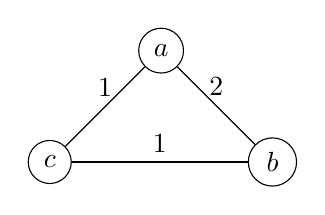
\begin{tikzpicture}[main/.style = {draw, circle},node distance=2cm]
        \node[main] (0) {$a$};
        \node[main] (1) [below right of=0] {$b$};
        \node[main] (2) [below left of=0] {$c$};

        \draw (0) -- node[midway, above] {$2$} (1);
        \draw (0) -- node[midway, above] {$1$} (2);
        \draw (1) -- node[midway, above] {$1$} (2);
\end{tikzpicture}
\caption{Visual representation of graph $G$.} \label{fig:graph1}
\end{figure}

We observe that for this graph there are 3 spanning trees:
$T_0 = \{(a,b), (a,c)\}$,
$T_1 = \{(a,b), (b,c)\}$,
$T_2 = \{(a,c), (b,c)\}$, with weights:

\[w(T) = \begin{cases}
        2 & \text{ for } T = T_0\\
        2 & \text{ for } T = T_1\\
        1 & \text{ for } T = T_2
        \end{cases}\]

Therefore we want to sample $T_0$ or $T_1$ each with probability 2/5, and $T_2$
with probability 1/5. But if we sample the trees by the method described above
(i.e., choosing edges propropotional to their weight---and for this graph just
pick the first two), then we get the following distribution:

\begin{align*}
(a,b), (a,c)\text{ with Pr }= 1/2 \cdot 1/2 = 1/4, (T_0 \text{ is selected})\\
(a,c), (a,b)\text{ with Pr }= 1/4 \cdot 2/3 = 1/6, (T_0 \text{ is selected})\\
(a,b), (b,c)\text{ with Pr }= 1/2 \cdot 1/2 = 1/4, (T_1 \text{ is selected})\\
(b,c), (a,b)\text{ with Pr }= 1/4 \cdot 2/3 = 1/6, (T_1 \text{ is selected})\\
(b,c), (a,c)\text{ with Pr }= 1/4 \cdot 1/3 = 1/12, (T_2 \text{ is selected})\\
(a,c), (b,c)\text{ with Pr }= 1/4 \cdot 1/3 = 1/12, (T_2 \text{ is selected})
\end{align*}

So we get:
\begin{align*}
\text{Pr}(T_0) = 1/4 + 1/6 = 10/24\\
\text{Pr}(T_1) = 1/4 + 1/6 = 10/24\\
\text{Pr}(T_2) = 1/12 + 1/12 = 1/6
\end{align*}

which is the wrong distribution (see above). We will see in the next section that
\emph{loop-erased random walks} are the key to sampling spanning trees.

\section{Loop-erased Random Walks}

The definitions in this section allow use of directed or undirected graphs. We
assume a stochastic transition matrix. If the edge weights of our graph do not
already form a stochastic matrix, we can obtain one by normalizing the weights
and (possibly) adding self-transitions for slack in probabilities. These
self-transitions will have no affect on the ensuing algorithms, for reasons that
will be clear shortly.

\begin{defn}
Given a stochastic $n\times n$ matrix $M$ corresponding to a graph $G = (V, E)$,
a \emph{random walk} is a sequence of vertices $v_i \in V$ such that
$\Prob(v_{i+1} = u) = M_{v_i,u}$.
\end{defn}

In other words, a random walk is just a run of a Markov chain whose state is a
single node and which can only transition to neighboring nodes.

A \emph{loop-erased random walk} (or \emph{self-avoiding random walk}) is
obtained by deleting the cycles of a random walk. That is, if in the course of
random walk, we find ourselves at a vertex for a second time the sequence is
deleted to the first visit of the node and we proceed as if it were that first
visit. Evidently, a loop-erased random walk must be finite since any repeating
nodes are deleted.

Some random walk algorithms measure their running time in
comparison to the \emph{cover time} of the graph, which is the expected number
of steps for a random walk (not loop-erased!) to reach all of the vertices the
first time.

% TODO hitting time

\section{Wilson's Algorithm}\label{wilson}
\subsection{Spanning tree with specified root node}
\begin{algorithm}
\caption{Wilson's algorithm for given root}
\label{alg:root}
\textbf{Input: }Graph $G=(V,E)$, Root $r \in V$ \\
\textbf{Output: }Spanning tree $T$
\begin{algorithmic}[1]
\STATE T = \{\}                   // Set of nodes which are in the tree
\STATE next = \{\}                // Map from nodes to their successor
\FOR{ each v in V}
\STATE $u \leftarrow v$
\WHILE{u not in T}\label{walk}
\STATE next[u] $\leftarrow$ samplesuccessor(u)
\STATE u $\leftarrow$ next[u]
\ENDWHILE \label{endwalk}
\STATE $u \leftarrow v$
\WHILE{u not in T} \label{adjoin}
\STATE T.add(u)
\STATE $u \leftarrow $next[u]
\ENDWHILE \label{endadjoin}
\ENDFOR
\STATE \textbf{return} next
\end{algorithmic}
\end{algorithm}

Wilson's algorithm for sampling a spanning tree with a specified root is given
in Algorithm~\ref{alg:root}. It works as follows:
\begin{itemize}
\item Initialize a tree to contain only the root.
\item For each node, perform a random walk until we hit the tree, and add that
path into the tree.
\item Return the resulting tree.
\end{itemize}


We note that the loop on lines~\ref{walk}-\ref{endwalk} implements the
loop-erased random walk in a subtle way.  Specifically, the erasure of a cycle is
\emph{not} a special case, in the sense that if we end up back where we started,
the successor we write down will overwrite the one that was previously there
anyway. This will orphan the rest of the links in the cycle (in the ``next''
array), but this is okay because these links cannot be read by the walk (which only
reads from ``next'' after writing to it) or the tree-adjoining section
(lines~\ref{adjoin}-\ref{endadjoin}) without first being rewritten by the
walk.

\subsection{Spanning tree with unspecified root}
\begin{algorithm}
\caption{Wilson's algorithm with unspecified root}
\label{alg:noroot}
\textbf{Input: }Graph $G=(V,E)$, probability $\epsilon$ \\
\textbf{Output: }Spanning tree $T$
\begin{algorithmic}
\STATE T = \{\}                   // Set of nodes which are in the tree
\STATE next = \{\}                // Map from nodes to their successor
\STATE num\_roots $\leftarrow$ 0
\FOR{$v$ in $V$}
\STATE $u \leftarrow i$
\WHILE{u not in T:}
\IF{chance($\epsilon$)}
\STATE next[u] $\leftarrow$ null
\STATE T.add(u)
\STATE num\_roots += 1
\IF{num\_roots = 2}
\STATE \textbf{return} Fail
\ENDIF
\ELSE
\STATE next[u] $\leftarrow$ samplesucc(u)
\STATE $u \leftarrow $next[u]
\ENDIF
\STATE $u \leftarrow v$
\ENDWHILE
\WHILE{u not in T} \label{adjoin2}
\STATE T.add(u)
\STATE $u \leftarrow $next[u]
\ENDWHILE
\ENDFOR
\STATE \textbf{return} next
\end{algorithmic}
\end{algorithm}

Wilson's algorithm for sampling a spanning tree without a specified root is
shown in Algorithm~\ref{alg:noroot}.

\section{Analysis of Wilson's Algorithm}

% Talk about markov chain proof

\section{Implementation}\label{imp}

We discuss our implementation of Wilson's Algorithm~\ref{alg:root} and Wilson's Algorithm~\ref{alg:noroot} along with an implementation of Kruskal's minimum spanning tree algorithm where the order on the edges being processed by the algorithm can be chosen according to three different strategies. These strategies are as follows. Firstly, we can order all edges by increasing edge cost to get the classic Kruskal's algorithm for minimum spanning trees. Secondly, we can output a random permutation of the edges to get a simple ``randomized'' version of Kruskal's algorithm. Thirdly, we can output a random ordering of edges where the probability that we pick a certain edge weight in the ordering is proportional to its edge weight and the edge weight of all unpicked edges so far. The last two options correspond to a naive approach for sampling a random spanning tree as outlined in Section~\ref{naive-attempt}.

Our implementation is written OCaml \texttt{4.11.0} and can be located in the \texttt{code} folder of the public GitHub repository \footnote{\url{https://github.com/mdmoeller/6820-finalproject}} for this project. We rely on the Dune \footnote{\url{https://github.com/ocaml/dune}} build system and Jane Street's Core \footnote{\url{https://opensource.janestreet.com/core/}} and Core\_Bench \footnote{\url{https://github.com/janestreet/core_bench}} libraries. Details on installing OCaml, the relevant dependencies and compiling the program can be found in the \texttt{README}. At a high-level, we have four modules.

\begin{itemize}
\item \texttt{Parser}: The parser takes as an input a file name that describes the undirected graph we would like to analyze and outputs a representation of that graph that we use for our algorithms. The input file describes a graph as two integers $n$ and $m$ which correspond to the number of vertices and edges of the graph respectively. Furthermore, the user enters $m$ lines in the format $i,j,p$ which is interpreted as an edge $(i,j)$ with weight $p$. The parser output a set of vertices $\{0,\dots,n-1\}$ and a adjacency list representation of the graph.
\item \texttt{Random\_tree}: This module implements Wilson's Algorithm~\ref{alg:root} and Wilson's Algorithm~\ref{alg:noroot} by taking as input a graph from the \texttt{Parser} module and running the corresponding algorithms as described in Section~\ref{wilson} and Wilson's original paper \cite{wilson}. The output is a set of edges which can then be written to a file where each edge is written to a line of the file.
\item \texttt{Kruskal}: The \texttt{Kruskal} module implements the three Kruskal algorithms described in the beginning paragraph of this section. Each algorithm takes as input a graph from the \texttt{Parser} module and sorts the edges accordingly. Then, Kruskal's minimum spanning tree algorithm is run and we output a set of edges that corresponds to a minimum spanning tree with respect to the order we picked. This module also has a function to generate all spanning trees of a given graph. The implementation is simple and takes exponential time, we generate all permutation of the edge set of a graph and for each permutation run Kruskal's minimum spanning tree algorithm. To remove isomorphic spanning trees we canonicalize each spanning tree by sorting the edge set using the lexicographic ordering on $\mathbb{N}\times\mathbb{N}$.
\item \texttt{Tester}: The \texttt{Tester} module runs a set of tests to measure the empirical distribution of the spanning trees found by each algorithm and the average running time of each algorithm. To achieve this the module exposes a single function called \texttt{test} that accepts as input a graph from the \texttt{Parser} module and an integer \texttt{iter} which is the number of times a given test should be run. Then, the test suite will generate all spanning trees using \texttt{Kruskal} and run each algorithm from \texttt{Random\_tree} and \texttt{Kruskal} \texttt{iter} many times. The results of the frequencies of each spanning tree is saved to a file while the running times of each algorithm is printed to the screen. This is actually a quirk of the Core\_Bench as it has limited functionality and we could find no other micro-benchmarking library for OCaml. (Here, micro-benchmarks are necessary as none of our tests on average run for more than a couple of hundred micro-seconds.)
\end{itemize}

The generated program, \texttt{tree\_sampler}, can be used to run either any one of the algorithms individually or the test suite. The test suite is used to run our experimental evaluation which we describe next.

\section{Evaluation}\label{eval}

We are motivated by the followign two questions.

\begin{enumerate}[1.]
\item What kind of experimental distributions do the two Wilson algorithms and the two naive sampling algorithms produce?
\item What are the performance overheads of using Wilson's algorithms versus naive sampling?
\end{enumerate}

To answer these questions we run our test suite as described in Section~\ref{imp} on two graphs. The first graph is the graph from Section~\ref{naive-attempt} and the second is a graph from the Wikipedia article titled `Kruskal's algorithm' \footnote{\url{https://en.wikipedia.org/wiki/Kruskal's_algorithm}} which describes Kruskal's minimum spanning tree algorithm and gives an example graph for the outcome. The purpose of testing on the first graph is clear, we wish to show that Wilson's two algorithms experimentally converge to the correct distribution while the naive sampling methods do not. The purpose of testing on the second graph is to run the algorithms on a graph with many spanning trees (this graph has $141$ of them after canonicalization) and could be considered a representative graph according to some criteria. In this case, the criteria is that it is in Wikipedia where almost everyone studying Kruskal's algorithm would with high likelihood have seen this article and the corresponding graph.

\subsection{Test 1}

We ran our test suite for $1$ million iterations for each algorithm on the graph from Section~\ref{naive-attempt}. Figure~\ref{fig1} gives the experimental distributions of running each of our algorithms $1$ million times. The deterministic Kruskal algorithm is only there as a sanity check as we expect it to provide the same result every iteration. The simple random Kruskal simply randomizes the edge order before running Kruskal's algorithm while the proportional random Kruskal makes sure to take into account the edge weights when picking a random order. The Wilson's algorithms are split into the without root case and the with root case where we try every possible root. The bars represent the three spanning trees where $T_0$, $T_1$ and $T_2$ correspond to the same spanning trees given in Section~\ref{naive-attempt}.

\begin{figure}[ht]
\includegraphics[scale=0.60]{fig1.png}
\caption{Experimental results of the testing suite on Graph~\ref{fig:graph1}}
\centering
\label{fig1}
\end{figure}

We see the expected results. The simple randomized Kruskal's algorithm almost splits the experimental distribution to $1/3$ probability that any of spanning trees are selected and this makes sense as in this algorithm we pick the ordering of edges without considering the weights on them. All of Wilson's algorithms produce distributions very close to the expected split of $400000$ for $T_0$ and $T_1$ and $200000$ for $T_2$ which means that the algorithms experimentally also converge to the theoretical distribution. Finally, the naive edge-weight proportional Kruskal's algorithm puts more weight on the $T_1$ spanning tree by picking it more than half of the experimental runs which deviates from the theoretical distribution by a lot. This experiment serves as experimental evidence to the observations we make in Section~\ref{naive-attempt} that naive sampling of spanning trees will not produce distributions that are proportional to the edge weights of a graph.

We also measure the runtime both in average micro-seconds to complete a single run of a given algorithm and the average of CPU cycles it took to complete a single run of a given algorithm. Table~\ref{tab1} gives the performance results of our experiments. Here, kc stands for thousands (kilo) of cycles.

\begin{table}[ht]
\centering
\begin{tabular}{||c c c||} 
\hline
Test name & Average Time & Average CPU cycles \\ [0.5ex] 
\hline\hline
\text{Deterministic Kruskal} & $1.17\mu$s & $1.63$kc \\ 
\hline
\text{Simple random Kruskal} & $1.28\mu$s & $1.78$kc \\
\hline
\text{Proportional random Kruskal} & $1.40\mu$s & $1.95$kc \\
\hline
\text{Wilson's algorithm without root} & $1.76\mu$s & $2.45$kc \\
\hline
\text{Wilson's algorithm with root 0} & $1.10\mu$s & $1.53$kc \\ 
\hline
\text{Wilson's algorithm with root 1} & $1.11\mu$s & $1.55$kc \\ 
\hline
\text{Wilson's algorithm with root 2} & $1.20\mu$s & $1.67$kc \\ [1ex] 
\hline
\end{tabular}
\caption{Performance results of the testing suite on Graph~\ref{fig:graph1}}
\label{tab1}
\end{table}

Here we see that Wilson's algorithm when a root is picked performs better than all of the other sampling algorithms and in some cases even better than the deterministic Kruskal's algorithm. This could be explained by the fact that Wilson's algorithm is quite simple and the normalization step is also straightforward as it involves dividing each node's out edge weights by the sum of all of it's out edge weights. The difference in the runtime of the randomized Kruskal algorithm's and the deterministic Kruskal's algorithm describes the cost of randomly selecting a set of edges as both the randomized Kruskal algorithms first randomizes the set of edges and then calls the same function as deterministic Kruskal. The worst performing algorithm is Wilson's unrooted algorithm and we believe that the overhead for this algorithm occurs from the $\epsilon$ chance parameter. The algorithm could run for many iterations while halving $\epsilon$ before it finds a spanning tree. Furthermore, the normalization step is a little more involved as it also requires adding self-loops to the input graph. Overall, we see that Wilson's algorithms also perform well compared to the naive algorithms by either outperforming naive algorithms or introducing an overhead of $37.5\%$ when compared to the simple naive algorithm $25.8\%$ when compared to the proportional naive algorithm and $46.7\%$ compared to Wilson's algorithm with root $2$. In the microsecond scale this overhead does not matter much but one may want to prefer the rooted version of Wilson's algorithm for larger graphs as this algorithm performs considerably better than all the other algorithms we tested.

\subsection{Test 2}\label{test2}

As mentioned previously, we use the graph from the Wikipedia article for `Kruskal's algorithm.' The graph has $7$ vertices and $11$ edges. Figure~\ref{fig:graph2} gives this graph.

\begin{figure}
\centering
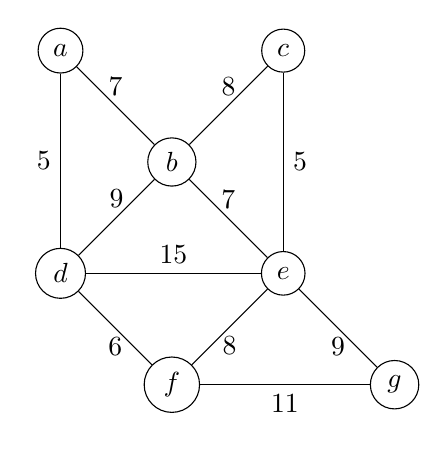
\begin{tikzpicture}[main/.style = {draw, circle},node distance=2cm]
        \node[main] (0) {$a$};
        \node[main] (1) [below right of=0] {$b$};
        \node[main] (2) [above right of=1] {$c$};
        \node[main] (3) [below left of=1] {$d$};
        \node[main] (4) [below right of=1] {$e$};
        \node[main] (5) [below right of=3] {$f$};
        \node[main] (6) [below right of=4] {$g$};

        \draw (0) -- node[midway, above] {$7$} (1);
        \draw (0) -- node[midway, left] {$5$} (3);

        \draw (1) -- node[midway, above] {$8$} (2);
        \draw (1) -- node[midway, above] {$9$} (3);
        \draw (1) -- node[midway, above] {$7$} (4);

        \draw (2) -- node[midway, right] {$5$} (4);

        \draw (3) -- node[midway, above] {$15$} (4);
        \draw (3) -- node[midway, below] {$6$} (5);

        \draw (4) -- node[midway, below] {$8$} (5);
        \draw (4) -- node[midway, below] {$9$} (6);

        \draw (5) -- node[midway, below] {$11$} (6);
\end{tikzpicture}
\caption{Visual representation of graph from Example section of Wikipedia article `Kruskal's algorithm.'} \label{fig:graph2}
\end{figure}

The graph in Figure~\ref{fig:graph2} has $6$ different roots and $141$ canonicalized spanning trees. This causes some cluttering if we were to present all the data in one chart so we choose to present the results for the following algorithms: simple randomized Kruskal, proportional randomized Kruskal, Wilson's algorithm with no root and Wilson's algorithm with the root chosen to be as $0$. The rest of the graphs comparing the expeted distribution to Wilson's algorithm where the root is chosen to be $1$ through $6$ can be found in the appendix Section~\ref{appendix1}. Figure~\ref{fig2} and Figure~\ref{fig3} presents the distributions obtained from our experiment. We use dashed vertical lines to delineate the experimental distrbitutions.

\begin{figure}[ht]
\includegraphics[scale=0.45]{fig2.png}
\caption{Experimental results of the testing suite on Graph~\ref{fig:graph2} comparing the expected distribution to the distributions produced by simple randomized Kruskal, Wilson's unrooted algorithm and Wilson's algorithm with root $0$}
\centering
\label{fig2}
\end{figure}

\begin{figure}[ht]
\includegraphics[scale=0.45]{fig3.png}
\caption{Experimental results of the testing suite on Graph~\ref{fig:graph2} comparing the expected distribution to the distributions produced by proportional randomized Kruskal}
\centering
\label{fig3}
\end{figure}

We see similar results to Test 1 but the distributions do not perfectly line up with our expectations. The simple randomized Kruskal's algorithms appears to be converging to a $1/141\times10^6$ distribution of occurrences for all spanning trees of the graph but there is clearly some skew as some of the spanning trees occur more frequently than other spanning trees. All of Wilson's algorithms appear to still produce distributions close to the expected distribution as both the unrooted and the root $0$ algorithms produce the same spikes in the experimental distribution as the expected distribution and behave very similarly. This observation is backed up by the fact that the other graphs in Section~\ref{appendix1} of the appendix also show similar behavior. This shows us that despite the instability in the simple randomized algorithm, Wilson's algorithms also experimentally produce similar distributions to the theoretical distribution. We see that the naive edge-wight proportional Kruskal's algorithm produces a wildly different distibution than the theoretical expected distribution by favoring certain spanning trees more than other with one spanning tree shooting up to a frequency of almost $250000$ while other spanning trees have either $0$ frequency or a very low frequency causing them to not appear on the graph as bars. Out of all the algorithms we ran, we see this naive proportional one to perform the worst in terms of the produced distribution. Overall, our experiment shows us that Wilson's algorithms are clearly in the experimental setting the best way to sample random spanning trees from a graph while the proportional sampling should be avoided while the simple randomized sampling tends to produce a uniform distribution but may not always tend that way.

Next, we also again measure the runtime both in average micro-seconds to complete a single run of a given algorithm and the average of CPU cycles it took to complete a single run of a given algorithm. Table~\ref{tab2} gives the performance results of these experiments.

\begin{table}[ht]
\centering
\begin{tabular}{||c c c||} 
\hline
Test name & Average Time & Average CPU cycles \\ [0.5ex] 
\hline\hline
\text{Deterministic Kruskal} & $3.44\mu$s & $4.79$kc \\ 
\hline
\text{Simple random Kruskal} & $3.99\mu$s & $5.55$kc \\
\hline
\text{Proportional random Kruskal} & $5.40\mu$s & $7.51$kc \\
\hline
\text{Wilson's algorithm without root} & $6.13\mu$s & $8.54$kc \\
\hline
\text{Wilson's algorithm with root 0} & $3.60\mu$s & $5.02$kc \\ 
\hline
\text{Wilson's algorithm with root 1} & $3.18\mu$s & $4.43$kc \\ 
\hline
\text{Wilson's algorithm with root 2} & $3.52\mu$s & $4.90$kc \\
\hline
\text{Wilson's algorithm with root 3} & $3.11\mu$s & $4.32$kc \\ 
\hline
\text{Wilson's algorithm with root 4} & $3.07\mu$s & $4.27$kc \\ 
\hline
\text{Wilson's algorithm with root 5} & $3.38\mu$s & $4.71$kc \\
\hline
\text{Wilson's algorithm with root 6} & $3.36\mu$s & $4.67$kc \\ [1ex] 
\hline
\end{tabular}
\caption{Performance results of the testing suite on Graph~\ref{fig:graph2}}
\label{tab2}
\end{table}

We again see that Wilson's algorithm when a root is picked performs better than all of the other algorithms including this time deterministic Kruskal except for when the picked root it $0$. There is some slight variation in the runtimes produced by picking a root where picking the root as $4$ performs the best while picking the root as $0$ performs the worst. We're not sure whether the picked root has any effect on the performance of the algorithm or whether the the variation in runtimes can be attributed to the fact that some of our random walks found the spanning tree faster by virtue of the randomness. The latter explanation seems likely as the literature we have looked at makes no mention at how picking the root would affect the runtime of the algorithm. We also again see that the unrooted Wilson's algorithm performs the worst by introducing an overhead of $53.6\%$ compared to simple randomized Kruskal, $13.5\%$ compared to proportional random Kruskal and $70.3\%$ compared to Wilson's algorithm where the root is picked to be $0$. We see that the overhead compared to proportional random Kruskal has gone down compared to Test 1 while the overheads compared to simple randomized Kruskal and rooted Kruskal have gone up. While we have not performed any further experimental analysis, our intuition would lead us to believe that the gaps between random simple Kruskal and rooted Kruskal compared to unrooted Kruskal would continue to increase as the graph size increases while the gap between proportional random Kruskal and unrooted Kruksal would stay steady with the unrooted algorithm performing the worst. We reiterate our observation from Test 1 that while at the microsecond scale itm ight not matter which algorithm we choose to use, in the larger graph case it is becoming even clearer that we may want to perfer the rooted algorithm unless we do not want to fix our sample to a single root.

\subsection{Potential Pitfalls of the Experimental Evaluation}

We discuss some of the underlying reasons that may have biased our results. Firstly, our implementation of Wilson's algorithms used more of OCaml's imperative constructs while the sampling steps of the naive randomized algorithm relied on more functional constructs. We do not have a strong reason to believe that this biased our experiments given that the type of computations we performed were near identical and the only aspect that changed between the implementations were the pragmatics (that is what we used to achieve what we wanted to). Furthermore, the OCaml compiler is known to be very good at optimization so the functional code could take advantage of those optimizations while the imperative code is restricted to a limited form. Nonetheless, we thought it was noteworthy to mention our implementation differences.

Secondly, we only performed two experiments on two graphs where each experiment ran a million times. While the number of runs is a good enough sample size, the number of graphs we considered is not. There could exist pathological cases, in terms of runtime, for all of our algorithms and we would either need to explore those theoretically or experimentally by considering a large database of graphs. In this case, comparing the distributions would not suffice and we would actually need to compute a distance between the experimental distributions and the theoretical ones. While with out experiments we can make some general observations that back-up our intuitions and our theoretical understanding of Wilson's algorithm, only a more robust testing suite can generalize those observations.

Finally, it became apparent to use that benchmarking in OCaml is difficult due to the lack of libraries on the platform. We could have rolled out our own solution but we were inexperienced in benchmarking OCaml code (for example, we would need a way to stabilize the garbage collector between runs) and so we settled on a library that does this for us. This library is a bit of black box for us at the moment making it difficult to evaluate how it works and how well it is at measuring the runtime of a piece of code.

\section{Conclusion}

We presented Wilson's algorithms on sampling a random spanning tree from a graph with a probability proportional to the weight of the sampled tree. We also presented two naive algorithms and theoretically showed why these algorithms do not sample spanning trees correctly. Finally, we carried out two experiments that justified our theoretical observations and showed that Wilson's rooted algorithms perform the best when sampling a random spanning tree.

Future work includes running more experiments where we measure the differences between distributions and considering whether Wilson's algorithms may have any pathological graphs that cause the algorithm to perform in its worst case runtime.

\printbibliography

\begin{appendices}\label{appendix}

\section{Additional graphs from Section~\ref{test2}}\label{appendix1}

\begin{figure}[ht]
\includegraphics[scale=0.40]{fig4.png}
\caption{Experimental results of the testing suite on Graph~\ref{fig:graph2} comparing the expected distribution to the distributions produced by Wilson's algorithm with roots $1$ through $3$}
\centering
\label{fig4}
\end{figure}

\begin{figure}[ht]
\includegraphics[scale=0.40]{fig5.png}
\caption{Experimental results of the testing suite on Graph~\ref{fig:graph2} comparing the expected distribution to the distributions produced by Wilson's algorithm with roots $4$ through $6$}
\centering
\label{fig5}
\end{figure}

\end{appendices}

\end{document}
